\section{Test}
\label{sec:related-test}

Software security initially started as part of software testing~\cite{sharma2017}.
Today, still, most security practices are done in the testing phase.
Some part of software security will always be reactive.
Like all other parts of computer science, security keeps advancing, and we will always know more tomorrow than we know today.

So while many novel security tools and practices have been introduced and proven to be effective, new practices generally do not replace old ones.
Instead, they are added to the arsenal of weapons that is available for development and security teams.
In this section, I describe new tools and practices as well as some traditional ones, as I believe they will stay relevant, even if new tools and practices are being introduced.

\subsection{Penetration testing}
Penetration testing is the practice of breaking into running software by attacking it.
Sometimes, the penetration tester has access to the source code to speed up this process.
It is a common practice used by many companies and usually external experts are hired to perform these tests~\cite{cruzes2017security,bsimm11}.
Since the penetration tester needs access to the running software this can only be done late in the \gls{sdlc}.
Already in the introduction, we addressed that relying on security experts does not scale well.
Furthermore, it does not integrate well in modern development strategies, where fast feedback cycles and frequent releases are key~\cite{securitytestingagile}.
Penetration testing does improve the security awareness of the developers, but does not cause any long-lasting change in development practices by itself~\cite{turpe2016penetration}.

\subsection{Code reviews}
To develop new features or fix bugs, a developer starts from a copy of the current codebase.
As other developers submit changed code, this copy gradually ceases to reflect the main (or master) version.
The longer development continues, the greater the risk of conflicts when merging work back into the main version.
A code review is a manual inspection of produced code that is performed when this work is merged back.
It is usually done by another developer than the original author but with that author present.
Code reviews also provide an educational aspect for the developer whose code is reviewed~\cite{futcher2008guidelines}.
The downside is that, similarly to penetration testing, it relies on internal or external experts and hence does not scale well.

\Gls{ci} tools are developed to merge the working copies of developers into a shared main version and automatically build and review code as frequently as possible.
A build server is usually set up for this purpose, that will build and test the code after every commit and report the results back to developers.
This testing is done with automated tools, such as static analysis tools.

\subsection{Static analysis}
Static analysis tools are well researched~\cite{li2017static,jovanovic2006pixy,livshits2005finding} and commonly used to detect vulnerabilities~\cite{cruzes2017security,bsimm9,bsimm11}.
Most tools can run automatically, and as a result are easily adapted in modern development strategies.
Static analysis tools vary from robust and time-consuming analyses such as Fortify~\cite{chess2004static} (battlecard~\ref{bc:fortify}) to light real-time analyses~\cite{brown2016build}.
In controlled experiments, static analysis tools proved to be more effective than penetration testing~\cite{Scandariato2013}.

\todo{whole list of tools that can be discussed}
Already mentioned in this work:
FindBugs
Fortify
Semgrep

As explained in this work, frequent testing is useful, but analyses of traditional security tools often run too long to be well-integrated in developer workflows.
These tools are often seen as a big inhibitor for the developer's productivity.
To mitigate this, a shift left movement is ongoing to apply them as early as possible in the \gls{sdlc}.

However, static analysis tools require sufficient code to be completed in order to detect vulnerabilities, and hence can usually not be used in a proactive manner.
By customizing the rules, some tools can be tailored to ignore context, which can speed up their analyses even if they were not designed with this in mind.
But even if local versions of the analyses perform well, they often do not provide fixes to resolve the discovered issues and hence do not enforce a paved path.
They can not be applied in a pro-active manner, like Sensei can.
An example of a tool that does provide fixes in the code review stage, is Tricorder~\cite{sadowski2015tricorder} (battlecard~\ref{bc:tricorder}), or its open-source version Shipshape (battlecard~\ref{bc:shipshape}).
Research with this tool showed that most developers go back to their \gls{ide} rather than use the code review tool to resolve the issues~\cite{sadowski2015tricorder}.

\subsection{IDE-based}
Because developers prefer to remediate problems in their \gls{ide}, and as part of the shift left movement, many static analysis tools are now available as \gls{ide} plugins as well.
For some tools no effort has been made to adapt them to better suit the developer.
They still perform identical analyses to the original tool, either remotely or locally.
Some tools even prevent the developer from making changes to the code while the scan is in progress.
Examples of plugins like this are Semgrep, FindBugs/Spotbugs
\todo{examples: Semgrep, FindBugs/SpotBugs}

Performing the full scan, however, often takes too long and as a result these tools are not very usable.
In an attempt to be more developer-friendly, other tools provide lightweight versions of the analyses.
\todo{examples: Fortify Security Assistant}

In this case, the plugin is often not able to detect the complete set of vulnerabilities that the original tool is capable of.
The goal is to provide faster feedback loops to the developer, with the drawback that some of the vulnerabilities will go unnoticed.
But by detecting a portion of the vulnerabilities earlier in the \gls{sdlc}, they become easier and less expensive to fix.
All the other vulnerabilities are still caught when the fully capable tool is used in later phases of the \gls{sdlc}

\subsection{Rule customization}
For these tools to be most effective, their rules should be tailored specific to the organization's coding standards and target vulnerabilities relevant to the organization's history~\cite{bsimm9,bsimm11}.
As described in this work, this also prevents false positives and \glspl{efp}, thus improving usability for developers and ensuring continued use of the tool.

To customizes the rules, different approaches exist.
In this section, they will be demonstrated with a rule to detect the use of the deprecated cryptographic algorithm \gls{des} in Java.
The insecure line of code that needs to be marked is shown in Listing~\ref{lst:useDES}.

\begin{lstlisting}[language={Java},caption={Insecure use of a deprecated cryptographic algorithm},label={lst:useDES},abovecaptionskip=-0.0pt,xleftmargin=15pt]
Cipher.getInstance("DES");
\end{lstlisting}

\subsubsection{API}
The first method of rule customization is through use of an \gls{api}.
These tools require the rule-writer to write code that extends the functionality of tool so that it performs additional analyses.
The tool, or sometimes only the extension itself, then needs to be built into a new executable that can be used to analyse software products.
For Shipshape it is even required to expose this executable as a service using a docker image\footurl{https://github.com/google/shipshape}.

Creating detectors through an \gls{api} allows sufficient flexibility, but makes it more complex to develop and test custom rules.
SpotBugs (battlecard~\ref{bc:SpotBugs}) is an example of a tool that uses an \gls{api} for rule customization by creating so-called third party ``detectors"~\cite{spotbugsapi}.
These detectors have to be implemented and compiled into a SpotBugs plugin.
FindSecBugs~\cite{findsecbugs} is a popular security plugin for SpotBugs.
A detector to mark use of the \gls{des} algorithm is already implemented by the FindSecBugs plugin.
In Listing~\ref{lst:detectDES-findbugs}, a snippet of the class \texttt{DesUsageDetector} is shown that implements this detector.
This code is copied from the \texttt{find-sec-bugs} project on GitHub\footnote{\url{https://github.com/find-sec-bugs/find-sec-bugs}}.
The class extends the abstract class \texttt{CipherDetector} that is also implemented by the plugin, and hence not an \gls{api} provided by the original tool.
To create a detector for such a relatively simple example, multiple files and many lines of code are already needed that require sufficient knowledge of the \glspl{api}.
While the creation of additional detectors is not as convenient as creating recipes with Sensei, at least the distribution of detectors through a plugin is convenient for users of the tool.

\begin{lstlisting}[language={Java},caption={Rule customization of SpotBugs is done through java code using their API.},label={lst:detectDES-findbugs},abovecaptionskip=-0.0pt,xleftmargin=15pt]
public class DesUsageDetector extends CipherDetector {
    ...
    @Override
    int getCipherPriority(String cipher) {
        cipher = cipher.toLowerCase();
        if (cipher.equals("des") || cipher.startsWith("des/")) {
            return Priorities.NORMAL_PRIORITY;
        }
        return Priorities.IGNORE_PRIORITY;
    }
    ...
}
\end{lstlisting}

\subsubsection{Custom query language}
To make customisation of rules easier, some tools provide a custom query language that makes abstractions of their \gls{api}.
They still require the rule writer to write code, but they usually provide more specific syntax to make the development of rules easier.

Code Query Language (CodeQL) is an example of such a query language.
It is a free and open-source semantic code analysis engine that is created with the goal to query code as if it were data.
It borrows syntactic elements from data query languages such as \gls{sql} as well as elements from Java.
CodeQL is used by the popular analysis platform Semmle (battlecard~\ref{bc:semmle}).
A CodeQL query that detects use of \gls{des} is shown in Listing~\ref{lst:detectDES-semmle}.
This query is less complex and easier to write compared to using an actual \gls{api}.
CodeQL provides an online ``Query console" that makes development of these queries easier.
It provides syntax highlighting and auto-completion.
With this console it is also possible to test the queries on several demo projects.
The available projects do not necessarily contain the code a rule-writer is targeting, as was the case for the example rule.
None of the 7 available projects is using the \gls{des} encryption algorithm.

\begin{lstlisting}[language={sql},caption={CodeQL query used by Semmle to find use of insecure algorithm DES.},label={lst:detectDES-semmle},abovecaptionskip=-0.0pt,xleftmargin=15pt]
import java
from MethodAccess call, Method method
where
  call.getMethod() = method and
  method.hasName("getInstance") and
  method.getDeclaringType().hasQualifiedName("javax.crypto", "Cipher") and
  method.getParameter(0).toString().regexpMatch("DES.*")
select call
\end{lstlisting}

The query language CxQuery by Checkmarx uses regular Java syntax.
It provides abstractions to iteratively filter results based on certain properties of the code.
Some knowledge of the \gls{api} is required, but Checkmarx provides  clear and easy to understand documentation that contains lots of examples.
The resulting query, shown in Listing~\ref{lst:detectDES-checkmarx}, is even shorter than the one for CodeQL and just as easy to understand.

\begin{lstlisting}[language={Java},caption={CxQuery query used by Checkmarx to find use of insecure algorithm DES.},label={lst:detectDES-checkmarx},abovecaptionskip=-0.0pt,xleftmargin=15pt]
result = All.FindByName("*getInstance*",11,11);
result = result.FindByParameterValue(0,"DES",BinaryOperator.IdentityEquality);
\end{lstlisting}

\subsubsection{Markup language}
Some tools allow customization of the rules through existing markup languages such \gls{xml} and \gls{yaml}.
SecureAssist~\cite{secureassist} is an example of such a tool~\cite{sastinide}. 
Additional rules can be added through a rule pack configurator.
Rules themselves are written in \gls{xml} format and the syntax is user-friendly and easily readable~\cite{secureassistruletutorial}.

In Listing~\ref{lst:SAexample}, an example rule is shown to discover uses of \gls{des}, as a comparison the same rule for the Sensei plugin is shown in Listing~\ref{lst:DES-Sensei}.
SecureAssist's rule syntax is similar to Sensei rules.
However, creating the rules requires learning their exact syntax, as no editor is provided, rules are created using any text-editor.
Sensei, on the other hand, provides a rule wizard, context-aware suggestions, and a \gls{gui} to edit the rules as well as live-previews in the \gls{ide}.
Sensei rules also support more comprehensive features such as the concept of untrusted variables and support for libraries.

\begin{lstlisting}[language={xml},caption={SecureAssist rule to discover use of DES},float,label={lst:SAexample},literate={\ \ }{{\ }}1,xleftmargin=12pt] 
<Match>
  <QualifiedName>javax.crypto.Cipher</QualifiedName>
  <Method>getInstance</Method>
  <Arguments>
    <Argument>
      <Index>0<Index>
      <Value>
        <ComparatorOperator>equals</ComparatorOperator>
        <ExpectedValue>DES</ExpectedValue>
        <ComparatorType>String</ComparatorType>
      </Value>
    <Argument>
  </Arguments>
</Match>
\end{lstlisting}

\begin{lstlisting}[language={yaml},caption={Sensei recipe to discover use of DES},float,label={lst:DES-Sensei},literate={\ \ }{{\ }}1,xleftmargin=12pt]
search:
  methodcall:
    type: javax.crypto.Cipher
    name: getInstance
    args:
      1:
        type: java.lang.String
        value: "DES"
availableFixes:
- name: "Change to use AES/GCM/NoPadding"
   actions:
   - rewrite:
         to: '{{qualifier}}.getInstance("AES/GCM/NoPadding")'
\end{lstlisting}

Like Sensei, Semgrep (battlecard~\ref{bc:semgrep}) uses \gls{yaml} and its rule format is also similar to that of Sensei.
While it is intended to be used as a testing tool, third-party plugins have been developed to use Semgrep in the \gls{ide}, making it potentially a great tool for supporting the paved path methodology.
A rule to detect and fix use of \gls{des} is shown in Listing~\ref{lst:Des-semgrep}.
It is important to note that Semgrep is the first tool discussed in this section that provides quick-fixes.
Besides the search pattern and the fix, the rule also includes metadata that is stored separately for Sensei recipes, such as the category, severity level, and descriptions.
Semgrep rules have a few advanced features, such as the concept of metavariables, an abstraction made available to track variables such as method names across the search pattern.
The metavariable \texttt{\$CIPHER} is used in the example to define the fix, this is more user-friendly than the templating language provided by Sensei where the rule-writer is required to know the appropriate name of the element in the \gls{ast}.

\begin{lstlisting}[language={yaml},caption={Semgrep rule to discover use of DES},float,label={lst:Des-semgrep},literate={\ \ }{{\ }}1,xleftmargin=12pt]
rules:
- fix: $CIPHER.getInstance("AES/GCM/NoPadding");
    id: des-is-deprecated
    languages:
      - java
    message: DES is considered deprecated. AES is the recommended cipher.
    metadata:
      category: security
      cwe: "CWE-326: Inadequate Encryption Strength"
      license: Commons Clause License Condition v1.0[LGPL-2.1-only]
      owasp: "A3: Sensitive Data Exposure"
    pattern: $CIPHER.getInstance("=~/DES/.*/");
    severity: WARNING
\end{lstlisting}

Semgrep provides a ``Playground" on their website that allows recipe-writers to develop and test rules.
In this editor, a rule-writer can use the ``Advanced" view which is similar to Sensei's code view.
A ``Simple" view is available as well, but it does not provide the same level of support as Sensei's \gls{ui} view does.
As shown in Figure~\ref{fig:semgrep-editor}, this view still requires the user to know and understand most of the \gls{yaml} syntax.
Testing is unfortunately not real-time, but is completed in several seconds.

\begin{sidewaysfigure}
  \centering
  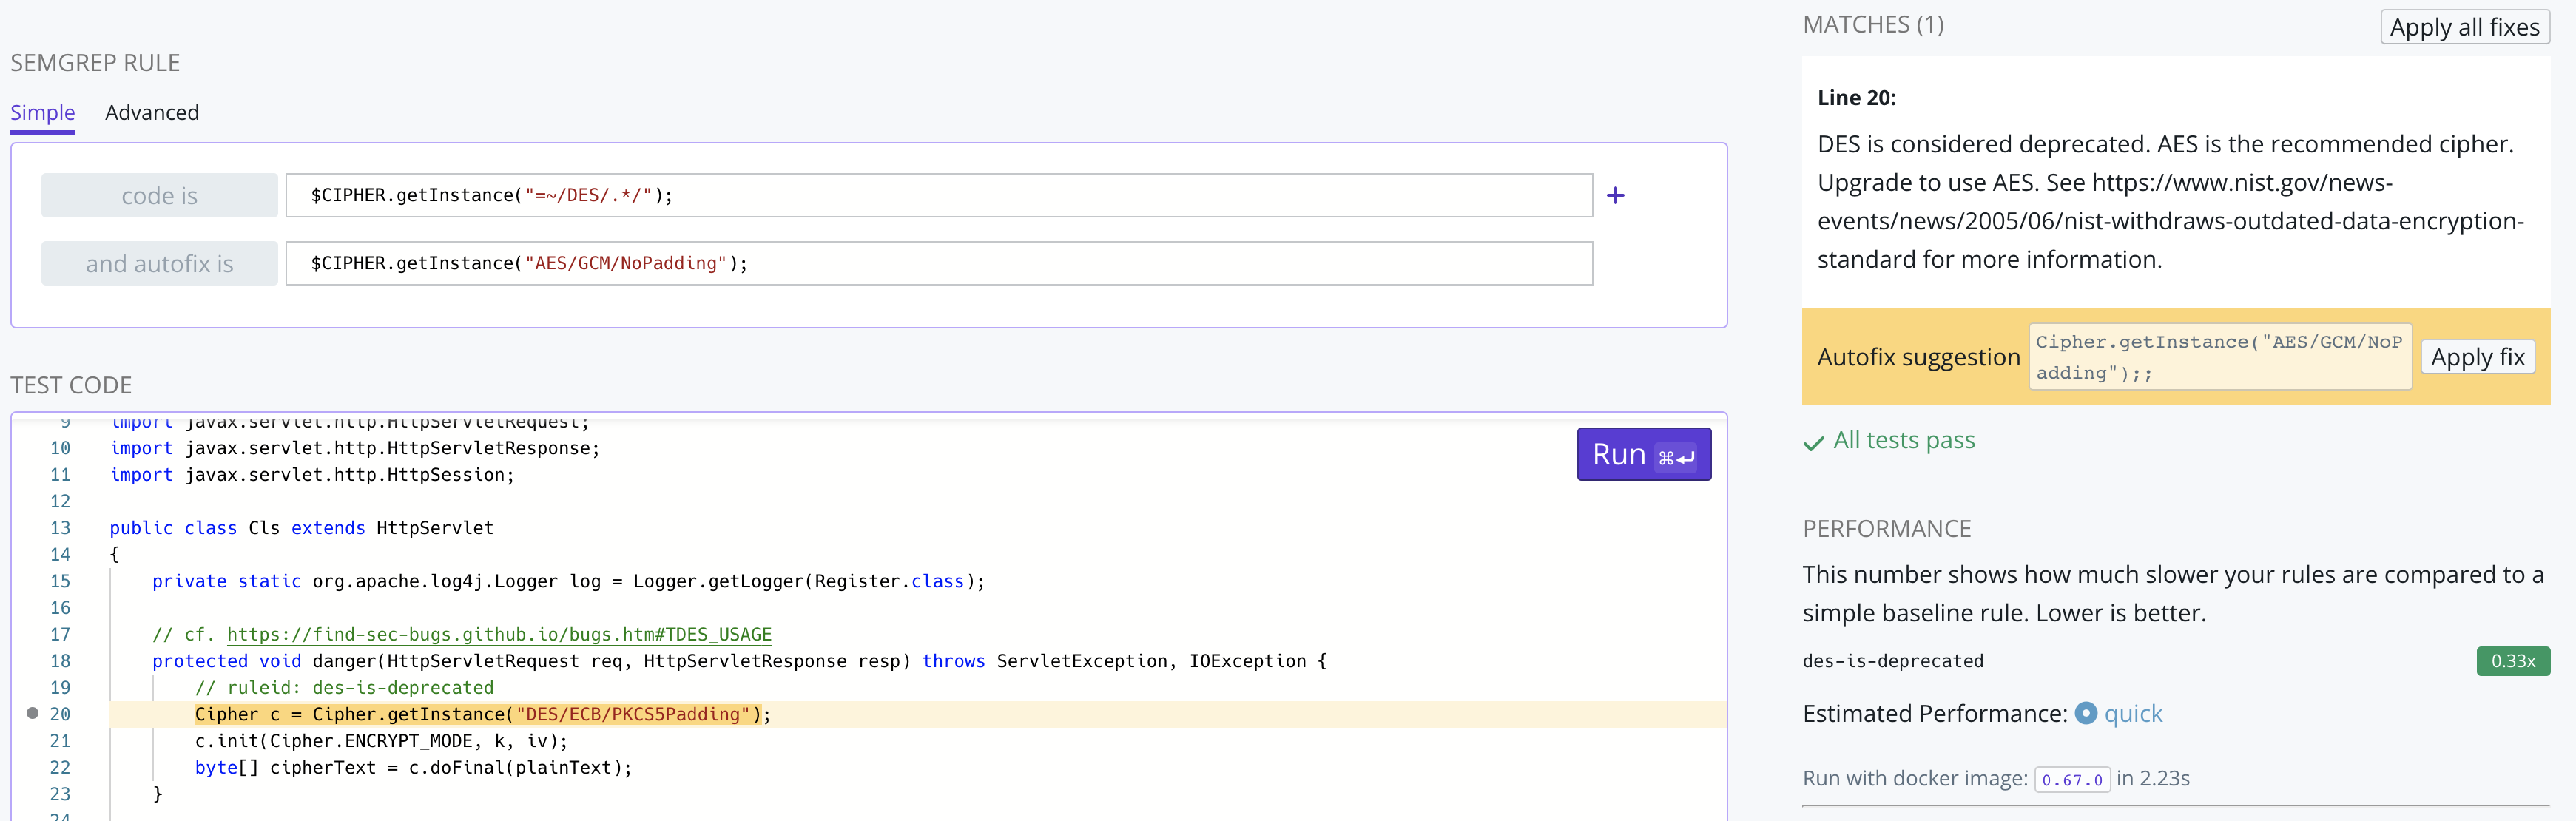
\includegraphics[width=\textwidth]{semgrep-editor.png}
  %\includegraphics[width=\textwidth,page=10]{04-tools/figures/figures2.pdf}
  \caption[Semgrep playground editor]{Semgrep's ``Simple" view in the Playground rule editor still requires use of the \gls{yaml} syntax.}
  \label{fig:semgrep-editor} 
\end{sidewaysfigure}

Semgrep also provides a few advanced features such as taint tracking which is similar to the concept of trusted input in Sensei.
To use taint tracking in a rule, sources and sinks need to be defined as well as optional sanitizers.
Since taint tracking requires a source to be specified, it functions differently to the trusted input of Sensei, where all input is untrusted by default.
Using metavariables it is possible to create a rule that prevents \glspl{efp} similarly to Sensei's trusted input. 
Listing~\ref{lst:metavariable} shows a rule to detect potential \gls{os} command injections, the analogous Sensei recipe is shown in Listing~\ref{lst:yamlrecipe}, but repeated here in Listing~\ref{lst:oscommand-sensei} for convenience.


\begin{minipage}[t]{0.9\linewidth}
\begin{lstlisting}[language={yaml},caption={Any commands passed on to the \texttt{exec} method that have not been retrieved through \texttt{getSafeCommand} will be marked.},label={lst:metavariable},xleftmargin=15pt]
rules:
- id: os-command
  patterns:
    - pattern: $RUNTIME.exec($COMMAND)
    - pattern-not-inside: |
        $COMMAND = getSafeCommand();
        ...
        $RUNTIME.exec($COMMAND);
  message: "Could lead to OS Command injection"
  languages: [java]
  severity: ERROR

\end{lstlisting}

\begin{lstlisting}[language={yaml},caption={Any input is untrusted by default except input retrieved through \texttt{getSafeCommand}. Untrusted input passed on to the \texttt{exec} methodcall will be marked.},label={lst:oscommand-sensei},xleftmargin=15pt]
search:
  methodcall:
    name: "exec"
    type: "java.lang.Runtime"
    args:
      1:
        type: "java.lang.String"
        containsUntrustedInput: true
        trustedSources:
        - methodcall:
            name: "getSafeCommand"
\end{lstlisting}
\end{minipage}